%!TEX root = ../Thesis.tex
%! Author = PR
%! Date = 27.05.2020


\section{Abläufe \textcolor{blue}{[Philipp Röring]}}

In \cref{fig:digitaler-briefkasten-pap} wird der grobe Ablauf der Anwendung in Form eines Programmablaufplans skizziert.
Dabei sollte beachtet werden, dass Maven nur während der Entwicklung der Anwendung relevant ist und nicht in der kompilierten
Anwendung enthalten ist.

\begin{figure}[hbt]
    \centering
    \begin{minipage}[t]{0.7\textwidth}
        \caption{Ablauf der Anwendung}
        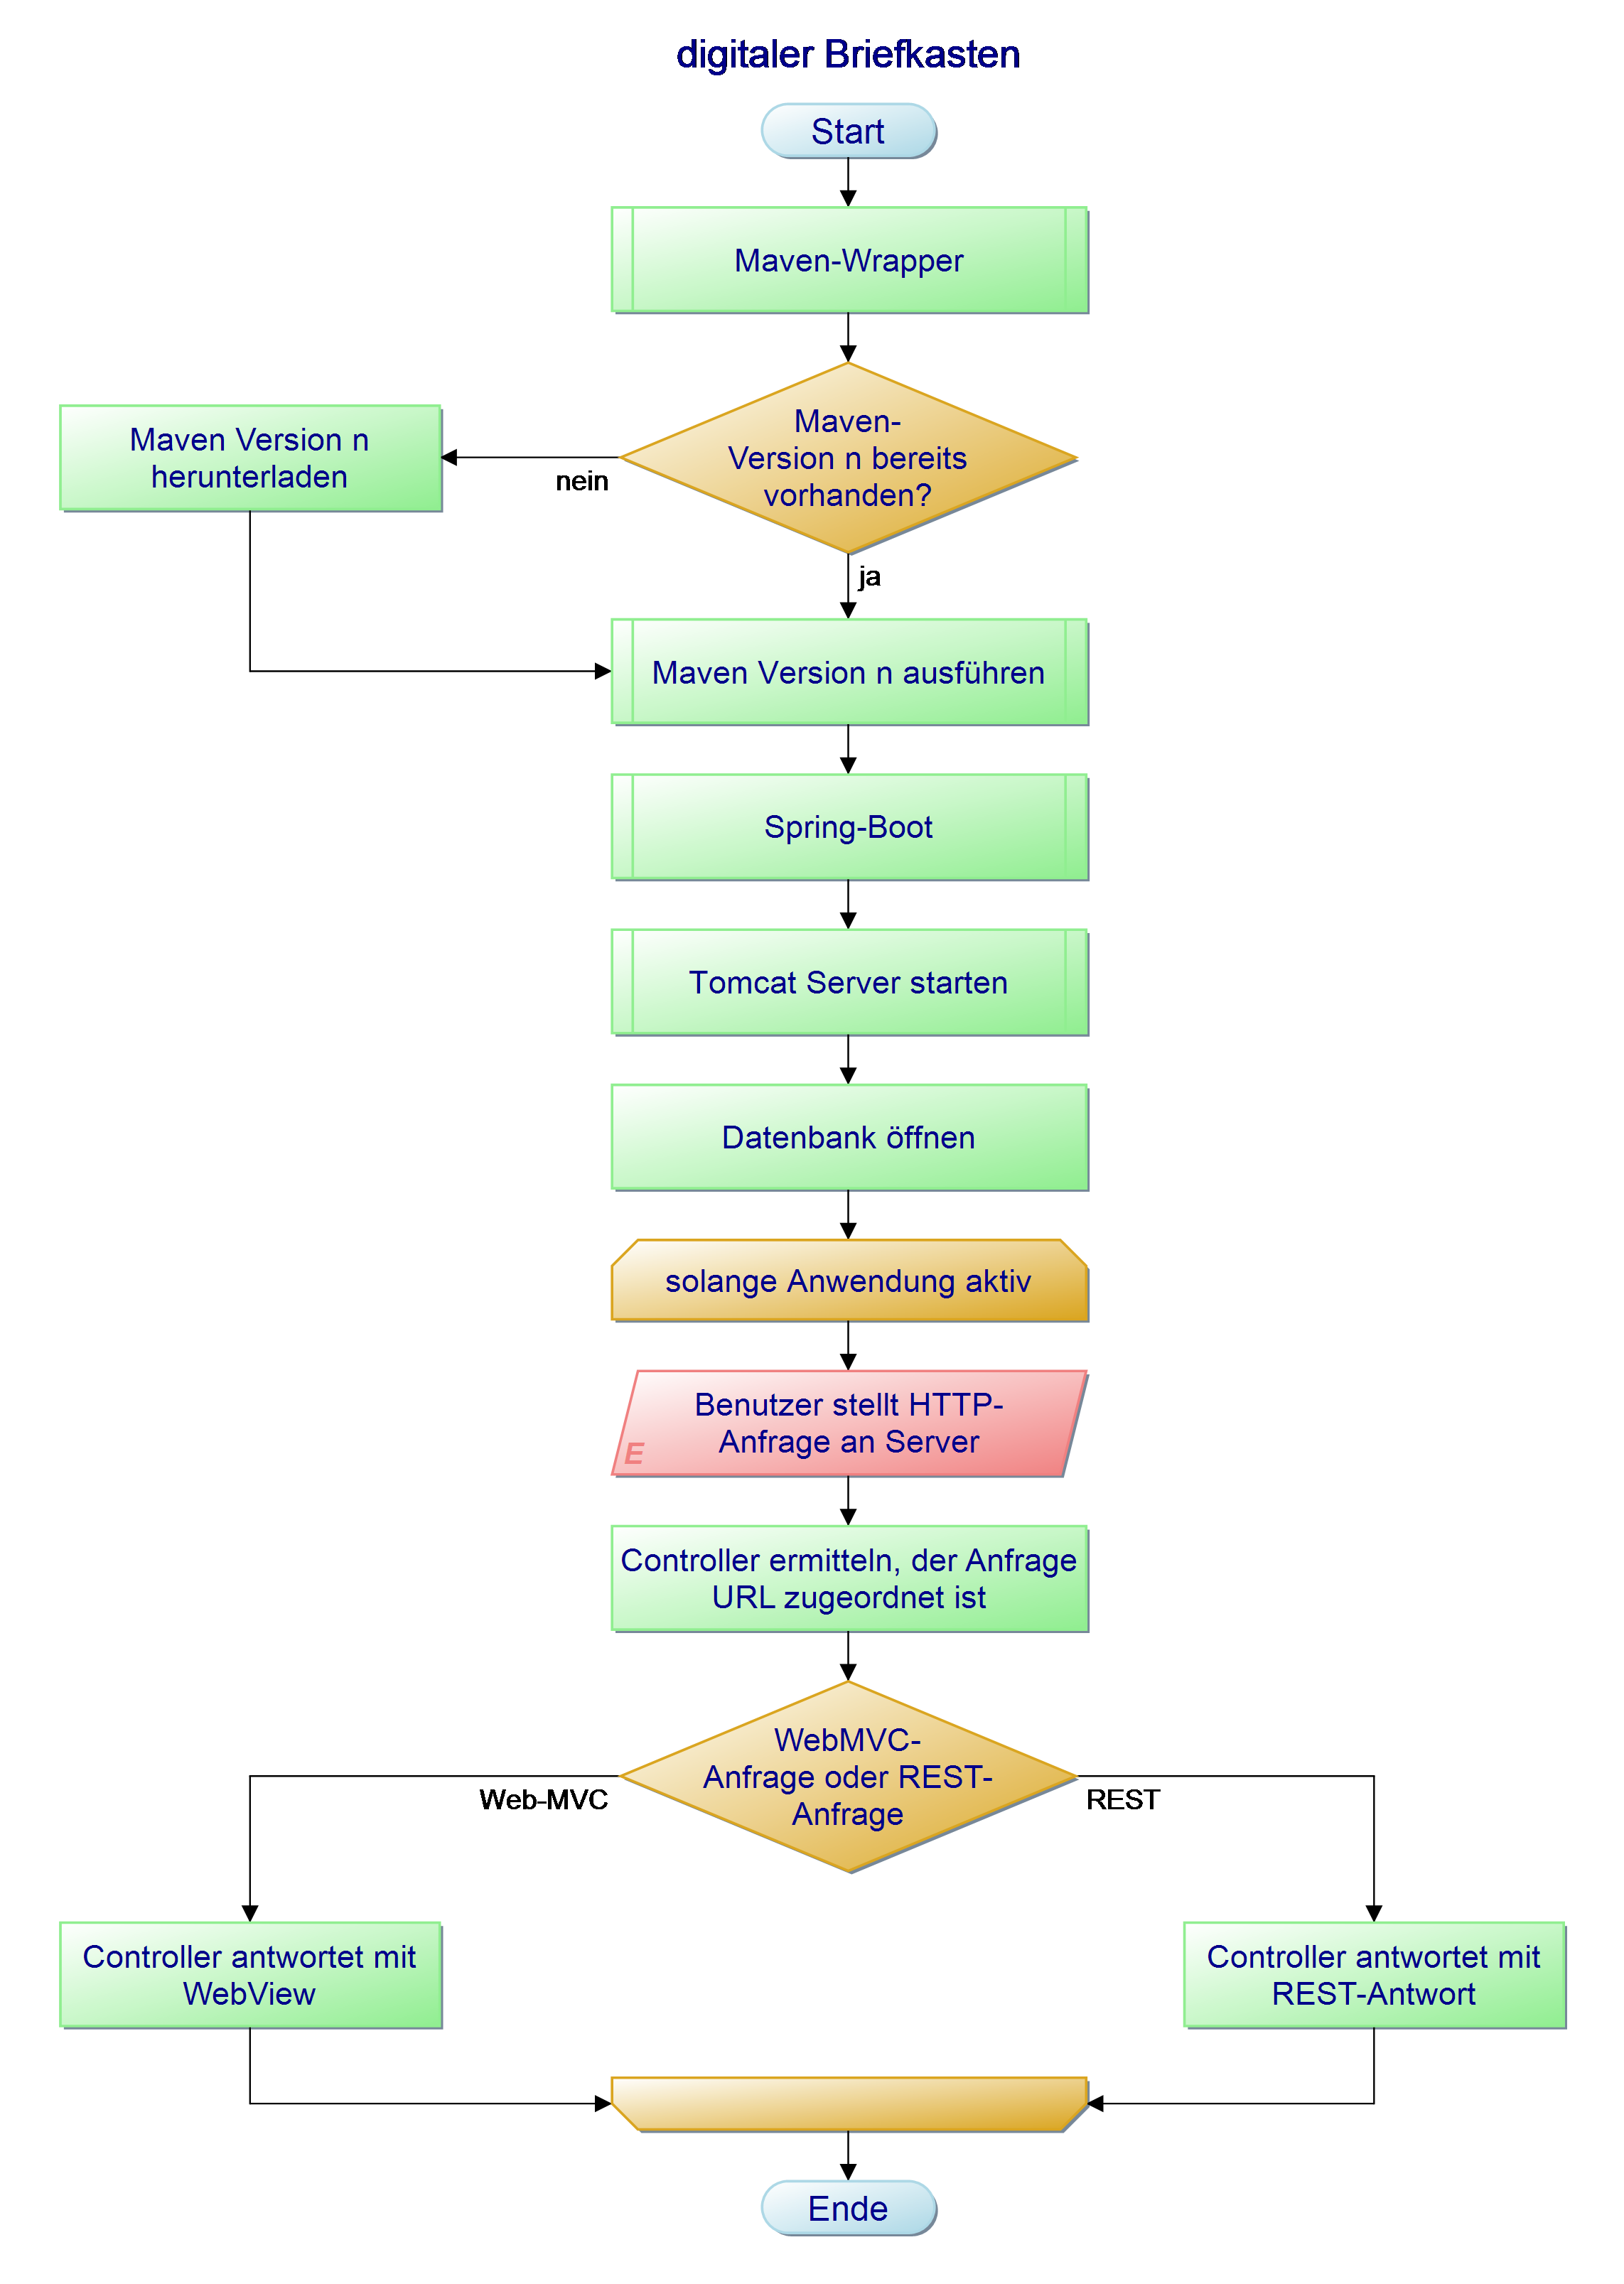
\includegraphics[width=1\textwidth]{img/digitaler-Briefkasten-pap.png}\\
        \source{Eigene Darstellung}
        \label{fig:digitaler-briefkasten-pap}
    \end{minipage}
\end{figure}







